\section{Te}
\subsection*{Material ID: mp-bghft}
\textbf{Constante Dieléctrica ($\epsilon_{total}$):} 64.81 \\[0.5em]
\begin{table}[h!]
\centering
\begin{tabular}{lcc}
\toprule
\textbf{Métrica} & \textbf{Lámina (Plate)} & \textbf{Cilindros (Rod)} \\
\midrule
Bandgaps ($a/\lambda$) & [0.711 - 0.711], [0.713 - 0.713], [0.724 - 0.724], [0.729 - 0.730], [0.732 - 0.738] & Ninguno \\
Resonancias & 36 & 36 \\
\bottomrule
\end{tabular}
\end{table}
\begin{figure}[H]
\centering
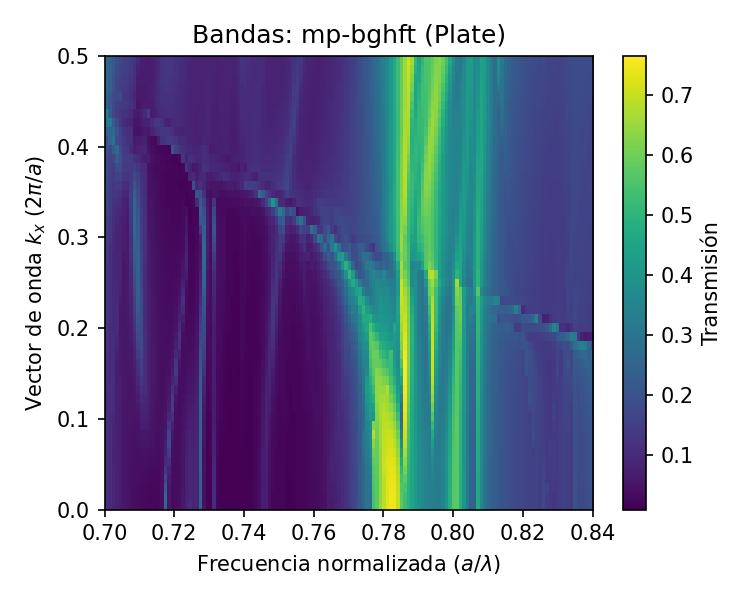
\includegraphics[width=0.48\textwidth]{figures/mp-bghft_plate.png}
\hfill
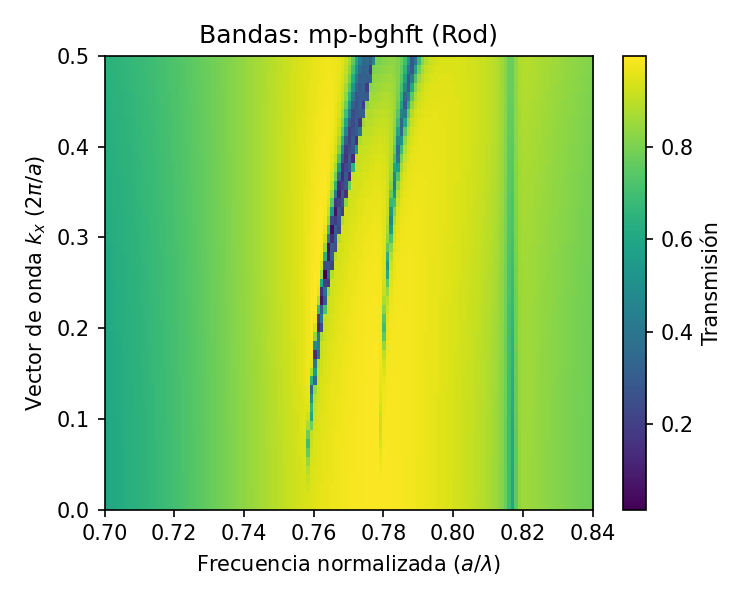
\includegraphics[width=0.48\textwidth]{figures/mp-bghft_rod.png}
\caption{Estructuras de bandas fotónicas para mp-bghft. Izquierda: Lámina. Derecha: Cilindros.}
\end{figure}
\vspace{1em}
\hrule
\vspace{1em}
\subsection*{Material ID: mp-t}
\textbf{Constante Dieléctrica ($\epsilon_{total}$):} 164.27 \\[0.5em]
\begin{table}[h!]
\centering
\begin{tabular}{lcc}
\toprule
\textbf{Métrica} & \textbf{Lámina (Plate)} & \textbf{Cilindros (Rod)} \\
\midrule
Bandgaps ($a/\lambda$) & [0.708 - 0.708], [0.804 - 0.805], [0.817 - 0.818] & [0.729 - 0.782] \\
Resonancias & 36 & 36 \\
\bottomrule
\end{tabular}
\end{table}
\begin{figure}[H]
\centering
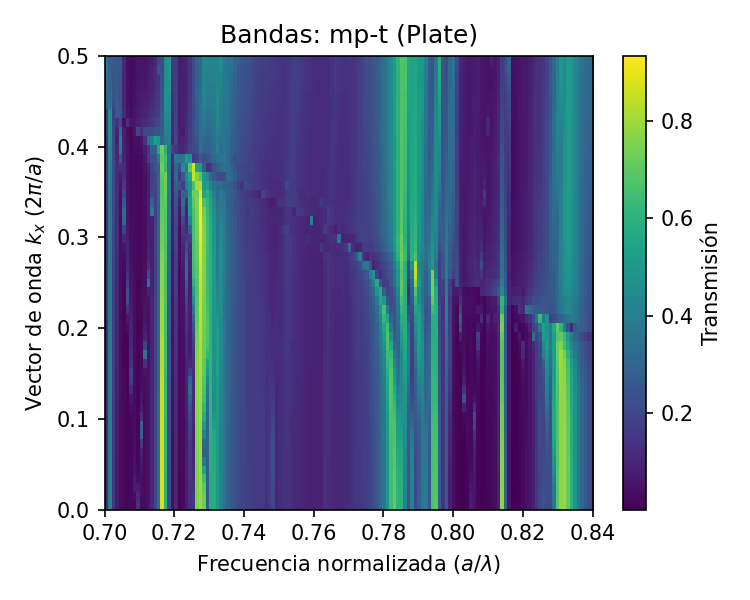
\includegraphics[width=0.48\textwidth]{figures/mp-t_plate.png}
\hfill
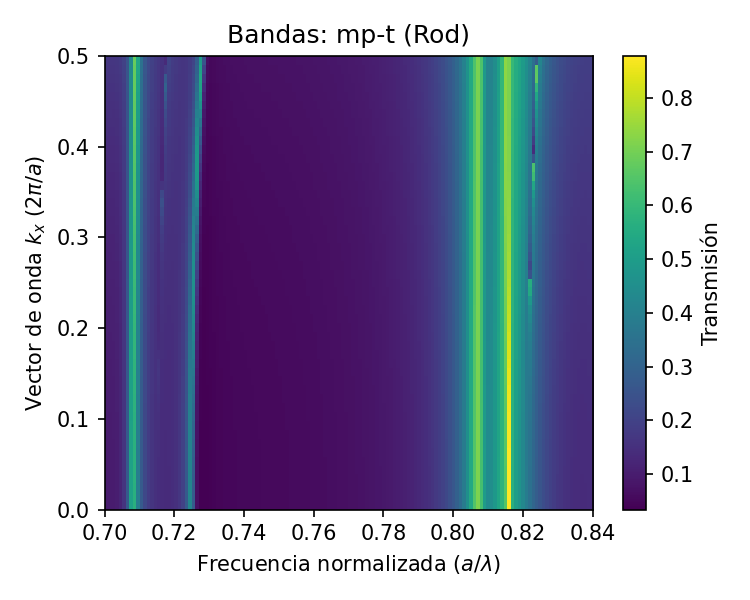
\includegraphics[width=0.48\textwidth]{figures/mp-t_rod.png}
\caption{Estructuras de bandas fotónicas para mp-t. Izquierda: Lámina. Derecha: Cilindros.}
\end{figure}
\vspace{1em}
\hrule
\vspace{1em}
\clearpage